\documentclass[10pt,a4paper]{article}
\usepackage{sketch} % See researchsketch.sty %
\usepackage{enumitem}
\usepackage[linesnumbered,ruled,vlined]{algorithm2e}
\usepackage{amsmath}
\usepackage{listings}
\usepackage{array}
\usepackage{tikz}
\usepackage{graphicx}
\usepackage{float}
\renewcommand{\lstlistingname}{\bfseries Program}
\makeatletter
\def\fnum@lstlisting{%
  \bfseries\lstlistingname
  \ifx\lst@@caption\@empty\else~\thelstlisting\normalfont\fi}%
\makeatother
\lstdefinestyle{myStyle}{
    belowcaptionskip=1\baselineskip,
    breaklines=true,
    frame=none,
    numbersep=5pt, 
    basicstyle=\footnotesize\ttfamily,
    keywordstyle=\bfseries\color{green!40!black},
    commentstyle=\bfseries\color{purple!60!black},
    identifierstyle=\color{blue},
}
\setenumerate[1]{itemsep=0pt, partopsep=0pt,topsep=5pt}
\setitemize[1]{itemsep=0pt, partopsep=0pt,topsep=5pt}
\author{1155189917}
\title{Research Note}
\pagestyle{fancy}
\renewcommand{\headrulewidth}{0pt}
\fancyhf{}
\rfoot{Page \thepage}
\date{\today}
\begin{document}
\noindent Convergence of \texttt{ASkewSGD}: A Quantization-Aware-Training Algorithm for Deep Neural Networks\\
Student: WONG, Hok Fong\hfill Research Progress Overview (Spring 2025)\\
\phantom{}\hrulefill
\setlength{\parindent}{0pt}
\section{Background} \marginpar{\small\textsf{\mbox{Jan 9, 2025}}}

We are interested in solving the optimization problem related to learning a quantized neural network (QNN),
\[\min_{\mathbf{w}\in\mathcal{Q}} \ell(\mathbf{w})\text{, where }\ell(\mathbf{w})=\mathbb{E}_{(\mathbf{x},y)\sim p_{\text{data}}} [\ell(f(\mathbf{x},\mathbf{w}), y)],\]
where $\ell:\mathbb{R}^d\to \mathbb{R}$ denotes the training loss, $\mathcal{Q}\subset \mathbb{R}^d$ is the set of quantization levels,
$d$ is the number of parameters in the neural network, $p_{\text{data}}$ is the training distribution \ref{1}.

We do not necessarily aim to solve the above (hard, combinational) optimization problem globally and optimally.
Instead, we want to find discrete weights $\mathbf{w}\in \mathcal{Q}$ that remain satisfactory when compared to the
non-quantized continuous weights \ref{2}.

\textbf{Goal.} Given a reasonably smooth function $\ell$, develop an algorithm with certain guarantees that converges
to a close-by quantized weight of a locally, or globally, optimal continuous weight with similar performance.

We turn to consider the smoothed sequence of interval-constrained optimization problems ($\mathcal{P}_\varepsilon$),
\[\min_{\mathbf{w}\in C_\varepsilon} \ell(\mathbf{w}), C_\varepsilon=\{\mathbf{w}\in \mathbb{R}^d: g_\varepsilon(\mathbf{w})\geq 0\},\]
where $\varepsilon$ is an annealing parameter that converges to zero.

Previously, Muehlebach and Jordan \ref{3} reformulated the position constraints into forward ``velocity'' constraints by considering a
linear and convex approximation of the original feasible set with the objective function satisfying the Mangasarian-Fromovitz condition.

\textbf{Definition (Mangasarian-Fromovitz Constraint Qualification).} $\forall \mathbf{x}\in \mathbb{R}^d$, $\exists \mathbf{w}\in \mathbb{R}^n$
s.t. $\nabla g_i(\mathbf{x})^\top \mathbf{w}>0$ for all $i\in I(\mathbf{x})$, where $I(\mathbf{x})=\{i\in \mathbb{Z}\bigm| g_i(\mathbf{x})\leq 0\}$.

By MFCQ, the set $V_\alpha(\mathbf{w})$, $V_\alpha(\mathbf{w})=\{\mathbf{v}\in\mathbb{R}^d: \nabla g_i(\mathbf{w})^\top \mathbf{v}\geq -\alpha g_i(\mathbf{w})\}$, is considered as an extension of the tangent cone outside of the feasible set, and is always a convex polyhedron.

\begin{algorithm}[H]
  \caption{Muehlebach-Jordan Algorithm}
  \For{$k=1,2,\ldots$}{
    $\mathbf{v}^{(k)} = \arg\min_{\mathbf{v}\in V_\alpha(\mathbf{w}^{(k)})} (1/2)\lVert \mathbf{v}+\nabla \ell(\mathbf{w}^{(k)})\rVert^2$.

    $\mathbf{w}^{(k+1)}=\mathbf{w}^{(k)}+\gamma_k \mathbf{v}^{(k)}$.
  }
\end{algorithm}


We note that $\alpha$ controls the trade-off betweeen two objectives: for large $\alpha$, the emphasis is on the convergence to the feasible set,
while for small $\alpha$, the focus is on reducing the objective function \ref{3}.

Muehlebach and Jordan's algorithm \ref{3} is then extended by Leconte et al. \ref{1} to the quantization-aware training algorithm \texttt{ASkewSGD}.

\textbf{Definition (Remoteness Measure of Iterates to the Quantization Set).} Let $\varepsilon\in[0,1]$, $w_i\in \mathcal{Q}_i, i\in [d]$,
where $\mathcal{Q}_i=\{q^{(1)}_i, \ldots, q^{(K_i)}_i\}$ are sets of quantization values defined coordinate-wise. We define the piecewise function
\begin{align*}\psi_{i}(w_i;\varepsilon):=\begin{cases}\varepsilon-(q_i^{(1)}-w_i)^2                    & w_i < q_i^{(1)},                                \\
             \varepsilon-(w_i-q_i^{(j-1)})^2(w_i-q_i^{(j)})^2 & q_i^{(j-1)}\leq w_i < q_i^{(j)}, j=2,\ldots, K, \\
             \varepsilon-(w_i-q_i^{(K_i)})^2                  & w_i \geq q_i^{(K_i)},\end{cases}
\end{align*} for all $w_i\in\mathbb{R}$ and $i\in [n]$.

We impose constraints on each parameter of the neural network, by setting $g_i(\mathbf{w})=\psi_i(w_i;\varepsilon)$. This then forms the feasible
set $C_\varepsilon$. Furthermore, $V_{\varepsilon, \alpha}=\{\mathbf{v}\in\mathbb{R}^d: v_i \psi'_i (w_i;\varepsilon)\geq -\alpha \psi_i(w_i;\varepsilon) \text{ for } i\in I_\varepsilon(\mathbf{w})\}$, where $I_\varepsilon(\mathbf{w})=\{i\in[d]: \psi_i(w_i;\varepsilon)\leq 0\}$.

\begin{algorithm}[H]
  \caption{\texttt{ASkewSGD} Algorithm for QNN Training}
  \For{$k=1,2,\ldots$}{
    Obtain a stochastic gradient $\widehat{\nabla\ell}(\mathbf{w}^{(k)})$.

    $\widehat{\mathbf{v}}^{(k)} = \text{clip}(\arg\min_{\mathbf{v}\in V_{\varepsilon,\alpha}(\mathbf{w}^k)} (1/2)\lVert \mathbf{v}+\widehat{\nabla \ell}(\mathbf{w}^{(k)})\rVert^2, M_c)$.

    $\mathbf{w}^{(k+1)}=\mathbf{w}^{(k)}+\gamma_k \widehat{\mathbf{v}}^{(k)}$.
  }
\end{algorithm}

The optimization problem \[\argmin_{\mathbf{v}\in V_{\varepsilon, \alpha}(\mathbf{w})} (1/2) \lVert \mathbf{v}+\mathbf{u}\rVert^2\] has an explicit solution:
\begin{align*}[\mathbf{s}_{\varepsilon, \alpha}(\mathbf{u},\mathbf{w})]_i:=\begin{cases}-u_i                                                    & \text{if }\psi_i(w_i;\varepsilon)>0 \text{ or }-u_i\cdot \psi_i'(w_i;\varepsilon)\geq -\alpha \psi_i(w_i;\varepsilon)\geq 0, \\
             -\alpha\psi_i(w_i;\varepsilon)/\psi'_i(w_i;\varepsilon) & \text{otherwise}.\end{cases}
\end{align*}

Furthermore, the set of stationary points are given by the Karush-Kuhn-Tucker condition:
\[\mathcal{Z}_\varepsilon:=\{\mathbf{w}\in C_\varepsilon: \mathbf{0}\in -\nabla \ell(\mathbf{w})-N_{C_\varepsilon}(\mathbf{w})\}.\]

\section{Existing Results} \marginpar{\small\textsf{\mbox{Jan 10, 2025}}}

\textbf{Assumption 1.} The function $\ell$ is $L_\ell$-smooth, i.e. \[\lVert \nabla\ell(\mathbf{x})-\nabla \ell(\mathbf{y})\rVert^2\leq L_\ell \lVert \mathbf{x}-\mathbf{y}\rVert^2.\]

\textbf{Assumption 2.} The function $\ell$ is $d$-times continuously differentiable.

\textbf{Assumption 3.} The stepsizes $(\gamma_k)_{k\geq 0}$ are positive, non-summable and square-summable, i.e. \[\sum\limits_{k=0}^\infty \gamma_k=\infty, \sum\limits_{k=0}^\infty \gamma_k^2<\infty.\]

\textbf{Note.} Under A1, the squared gradient of the function $\ell$ is bounded by $L_\ell$.

\textbf{Theorem 1.} (Leconte et al., \ref{1}) Assume A1-A3 and $0<\varepsilon\leq \inf_{1\leq i\leq d}\inf_{1\leq j< K_i} \lvert q^{(j)}_i - q^{(j+1)}_i\rvert^4/16$, where $\{q^{(j)}_i\}$ are the quantization levels, $\ell(\mathbf{w}^{(k)})$ converges and $\lim_{k\to\infty} \text{d}(\mathbf{w}^{(k)}, \mathcal{Z}_\varepsilon)=0$ almost surely.

\textbf{Lemma 1.} (Leconte et al., \ref{1}) Under A3, it holds that $\lim\sup_{k\to\infty} \text{d}(\mathbf{w}^{(k)}, C_\varepsilon)=0$ almost surely.

\section{Current Work} \marginpar{\small\textsf{\mbox{Jan 10, 2025}}}

\textbf{Assumption 4.} $\gamma_k=\gamma_0/(k+1)$, where $\gamma_0>0$. We note that this is a special case of A3.

\textbf{Theorem 2.} (Our work) Assume A1, A4, and $0<\varepsilon\leq \inf_{1\leq i\leq d}\inf_{1\leq j< K_i} \lvert q^{(j)}_i - q^{(j+1)}_i\rvert^2/4$, where $\{q^{(j)}_i\}$ are the quantization levels, $\lim_{k\to\infty} \mathbb{E}[\lVert \mathbf{v}^{(k)}\rVert_2^2]=\mathbf{0}$ almost surely, where $\mathbf{v}$ is the deterministic version of the stochastic iterative update term $\widehat{\mathbf{v}}$.

\textbf{Definition (Categorization of the Update Direction).} We categorize the update direction $\mathbf{v}^{(k)}$ into two types: the gradient direction ($\nabla\ell(\mathbf{w})$ or $\widehat{\nabla\ell}(\mathbf{w})$) and the skewed pushing force ($\mathbf{u}$ or $\widehat{\mathbf{u}}$) directed toward the feasible set.
Let $T_\varepsilon(\mathbf{w})$ (and $T_\varepsilon(\mathbf{w}, \widehat{\nabla\ell}(\mathbf{w}))$ denoted as $\hat{T}_\varepsilon$) be the set of indices containing the coordinates taking an update given by the constraint $g_i(\textbf{w})$ for the deterministic case (and for the stochastic case).

\textbf{Definition (Quadratic Remoteness Measure of Iterates to the Quantization Set).} Let $\varepsilon\in[0,1]$, $w_i\in \mathcal{Q}_i, i\in [d]$,
where $\mathcal{Q}_i=\{q^{(1)}_i, \ldots, q^{(K_i)}_i\}$ are sets of quantization values defined coordinate-wise. We define the piecewise function
\begin{align*}\psi_{i}(w_i;\varepsilon):=\begin{cases}\varepsilon-(q_i^{(1)}-w_i)                  & w_i < q_i^{(1)},                                  \\
             \varepsilon-(q_i^{(j-1)}-w_i)(w_i-q_i^{(j)}) & q_i^{(j-1)}\leq w_i < q_i^{(j)}, j=2,\ldots, K_i, \\
             \varepsilon-(w_i-q_i^{(K_i)})                & w_i \geq q_i^{(K_i)},\end{cases}
\end{align*} for all $w_i\in\mathbb{R}$ and $i\in [n]$.

\textbf{Note.} We specifically consider the low-order form for simplifying the computations in Lemma 2.

\marginpar{\small\textsf{\mbox{Jan 19, 2025}}}
\textbf{Lemma 2.} Fix an arbitrary $0<\varepsilon\leq \inf_{1\leq i\leq d}\inf_{1\leq j<K_i} \lvert q_i^{(j)} - q_{i}^{(j+1)}\rvert^2/4$, where $\{q_i^{(j)}\}$ are the quantization levels. Denote $[q_-, q_+]$ as the set $C_{\varepsilon,i}\cap [(q_i^{(j)}+q_i^{(j-1)})/2, (q_i^{(j)}+q_i^{(j+1)})/2)$, where $C_{\varepsilon,i}$ is the projection of $C_\varepsilon$ on the $i$-th coordinate.
Let $\varepsilon_1>0$ and $\varepsilon_2<0$ be some small perturbations on a quantization level. Then,
\begin{enumerate}[label=(\alph*)]
  \item $$\left\lvert \frac{-\alpha\psi_i(q_++\varepsilon_1;\varepsilon)}{\psi'_i(q_++\varepsilon_1;\varepsilon)}\right\rvert \leq \alpha K_1\varepsilon_1;$$
  \item $$\left\lvert \frac{-\alpha\psi_i(q_-+\varepsilon_2;\varepsilon)}{\psi'_i(q_-+\varepsilon_2;\varepsilon)}\right\rvert \leq -\alpha K_2\varepsilon_2,$$
\end{enumerate}
for some constants $K_1, K_2>0$ determined solely by $\varepsilon, \varepsilon_1$ and the quantization levels.

\textbf{Proof.} By symmetry, we only need to prove the first statement. Note that \begin{equation}
  \psi_i(q_+;\varepsilon)=\varepsilon-(q_+-q_i^{(j-1)})(q_i^{(j)}-q_+)=0.
\end{equation}
Also, \begin{equation}
  \psi_i'(w;\varepsilon)=2w-q_i^{(j+1)}-q_i^{(j)}.
\end{equation}

Using (1),
$$\begin{aligned}
    \psi_i(q_++\varepsilon_1;\varepsilon) & =\varepsilon+(q_++\varepsilon_1-q_i^{(j)})(q_++\varepsilon_1-q_i^{(j+1)})                               \\
                                          & =\varepsilon+(q_+-q_i^{(j)})(q_+-q_i^{(j+1)})+\varepsilon_1(2q_+-q_i^{(j+1)}-q_i^{(j)})+\varepsilon_1^2 \\
                                          & =\varepsilon_1(2q_+-q_i^{(j+1)}-q_i^{(j)})+\varepsilon_1^2<0.
  \end{aligned}$$

Since $\varepsilon_1>0$, we have $\psi_i'(q_++\varepsilon_1;\varepsilon)<0$ by (2). Then,
$$\begin{aligned}\left\lvert \frac{-\alpha\psi_i(q_++\varepsilon_1;\varepsilon)}{\psi'_i(q_++\varepsilon_1;\varepsilon)}\right\rvert&=\frac{\alpha(\varepsilon_1(2q_+-q_i^{(j)}-q_i^{(j+1)}))}{(2q_+-q_i^{(j)}-q_i^{(j+1)})+2\varepsilon_1}\\&=\alpha\varepsilon_1-\frac{\alpha\varepsilon_1^2}{(2q_+-q_i^{(j)}-q_i^{(j+1)})+2\varepsilon_1}.\end{aligned}$$

Let $\varepsilon_1\leq -(2q_+-q_i^{(j)}-q_i^{(j+1)})/K$ and $K>2$, then $$\left\lvert \frac{-\alpha\psi_i(q_++\varepsilon_1;\varepsilon)}{\psi'_i(q_++\varepsilon_1;\varepsilon)}\right\rvert\leq \alpha\varepsilon_1-\frac{\alpha\varepsilon_1}{-K+2}=\alpha\varepsilon_1\frac{K-1}{K-2}.$$\qed

\phantom{}\\\phantom{}\\

\textbf{Corollary 1.} We note that Leconte's proof on the convergence to the feasible set $C_\varepsilon$ is not specific to the remoteness measure. In finite time, the skewed update direction toward the feasible set $\mathbf{u}^{(k)}$ will become small enough. Formally, \[\lim_{k\to\infty} \mathbf{u}^{(k)}\to 0.\]

\textbf{Proof.} By Lemma 1, $\lim\sup_{k\to\infty} \text{d}(\mathbf{w}^{(k)}, C_\varepsilon)=0$ almost surely. Using the $\epsilon$-$N$ definition of limits, $\forall \epsilon_1>0$, $\exists N\in\mathbb{N}$ s.t. $\forall k\geq N$, $\text{d}(\mathbf{w}^{(k)}, C_\varepsilon)<\epsilon_1$. Then, the perturbation of a single coordinate must also be bounded by $\varepsilon_1$. By Lemma 2, for $\varepsilon_1$ small enough we can fix a constant $K=-(2q_+-q_i^{(j+1)}-q_i^{(j)})/\varepsilon_1$ such that $$\left\lvert u^{(k)}_i \right\rvert\leq \alpha\varepsilon_1\frac{K-1}{K-2}.$$ Hence, we also have that \[\lim_{k\to\infty} \mathbf{u}^{(k)}\to 0.\]\qed
\newpage
\subsection{Step 1: Full Gradient Convergence Proof}\hfill\\

\textbf{Goal.} We prove that the full gradient oracle ensures the convergence of the update direction $\mathbf{v}\to \mathbf{0}$.

\textbf{Proof.} First, apply the descent lemma on the $L_\ell$-smooth function $\ell$. Then, we discuss the two cases of the update coordinate-wisely. We obtain the following inequality:

\begin{align*}\ell(\mathbf{w}^{(k+1)}) & \leq \ell(\mathbf{w}^{(k)})+\gamma_k (\mathbf{v}^{(k)})^\top \nabla \ell(\mathbf{w}^{(k)})+\frac{\gamma_k^2 L_\ell}{2}\lVert \mathbf{v}^{(k)}\rVert_2^2                                                                      \\
                                       & =\ell(\mathbf{w}^{(k)})+\gamma_k \sum\limits_{i\in T_\epsilon(\mathbf{w}^{(k)})} u_i^{(k)} [\nabla \ell(\mathbf{w}^{(k)})]_i-\gamma_k \sum\limits_{i\notin T_\epsilon(\mathbf{w}^{(k)})} [\nabla \ell(\mathbf{w}^{(k)})]_i^2 \\
                                       & \quad +\frac{\gamma_k^2 L_\ell}{2}\sum\limits_{i\in T_\epsilon(\mathbf{w}^{(k)})} (u_i^{(k)})^2+\frac{\gamma_k^2 L_\ell}{2}\sum\limits_{i\notin T_\epsilon(\mathbf{w}^{(k)})} [\nabla \ell(\mathbf{w}^{k})]_i^2.
\end{align*}

We further assume that $1-\gamma_k L_\ell/2>0$, i.e. $\gamma_k<2/L_\ell$, then
\begin{align*}
  \ell(\mathbf{w}^{(k+1)}) & \leq \ell(\mathbf{w}^{(k)})-\frac{\gamma_k}{2}\sum\limits_{i\notin T_\epsilon(\mathbf{w}^{(k)})} [\nabla \ell(\mathbf{w}^{(k)})]_i^2+\gamma_k \sum\limits_{i\in T_\epsilon(\mathbf{w}^{(k)})} u_i^{(k)} [\nabla \ell(\mathbf{w}^{(k)})]_i +\frac{\gamma_k^2 L_\ell}{2}\sum\limits_{i\in T_\epsilon(\mathbf{w}^{(k)})} (u_i^{(k)})^2.
\end{align*}

Using the $\varepsilon$-$N$ definition of limits, fix $\epsilon_1>0$, and apply Lemma 1 to obtain $N$ for the forthcoming argument.

Since the gradient of $\ell$ is bounded by $L_\ell$, and the skewed update direction $\textbf{u}^{(k)}$ is bounded by $C\varepsilon_1$ due to Lemma 2, we have
\begin{align*}
  \ell(\mathbf{w}^{(k+1)}) & \leq \ell(\mathbf{w}^{(k)})-\frac{\gamma_k}{2}\sum\limits_{i\notin T_\epsilon(\mathbf{w}^{(k)})} [\nabla \ell(\mathbf{w}^{(k)})]_i^2+\gamma_k \sum\limits_{i\in T_\epsilon(\mathbf{w}^{(k)})} C\varepsilon_1 L_\ell +\frac{\gamma_k^2 L_\ell}{2}\sum\limits_{i\in T_\epsilon(\mathbf{w}^{(k)})} (C\varepsilon_1)^2 \\
                           & \leq \ell(\mathbf{w}^{(k)})-\frac{\gamma_k}{2}\sum\limits_{i\notin T_\epsilon(\mathbf{w}^{(k)})} [\nabla \ell(\mathbf{w}^{(k)})]_i^2+\gamma_k n C\varepsilon_1 L_\ell +\frac{\gamma_k^2 L_\ell}{2}n C^2\varepsilon_1^2
\end{align*}
by $\varepsilon_1$ small enough and $C$ be given according to Corollary 1.

Rearranging the inequality and adding the squared skewing term yields
\begin{align*}
  \frac{\gamma_k}{2}\sum\limits_{i\notin T_\epsilon(\mathbf{w}^{(k)})} [\nabla \ell(\mathbf{w}^{(k)})]_i^2                                                                                    & \leq \ell(\mathbf{w}^{(k)})-\ell(\mathbf{w}^{(k+1)})+\gamma_k n C\varepsilon_1 L_\ell +\frac{\gamma_k^2 L_\ell}{2}n C^2\varepsilon_1^2                                               \\
  \frac{\gamma_k}{2}\sum\limits_{i\notin T_\epsilon(\mathbf{w}^{(k)})} [\nabla \ell(\mathbf{w}^{(k)})]_i^2+\frac{\gamma_k}{2}\sum\limits_{i\in T_\varepsilon(\mathbf{w}^{(k)})} (u_i^{(k)})^2 & \leq \ell(\mathbf{w}^{(k)})-\ell(\mathbf{w}^{(k+1)})+\gamma_k n C\varepsilon_1 L_\ell +\frac{\gamma_k^2 L_\ell}{2}n C^2\varepsilon_1^2+\frac{\gamma_k}{2}\cdot n(C^2\varepsilon^2_1) \\
  \frac{\gamma_k}{2}\sum\limits_{i\notin T_\epsilon(\mathbf{w}^{(k)})} [\nabla \ell(\mathbf{w}^{(k)})]_i^2+\frac{\gamma_k}{2}\sum\limits_{i\in T_\varepsilon(\mathbf{w}^{(k)})} (u_i^{(k)})^2 & \leq \ell(\mathbf{w}^{(k)})-\ell(\mathbf{w}^{(k+1)})+D\varepsilon_1,
\end{align*}
where $D$ is picked such that $D>\gamma_k n C(L_\ell+\gamma_k L_\ell C\varepsilon_1/2+C\varepsilon_1/2)$.

Note that the left hand side of the inequality is simply $\gamma_k/2 \lVert \mathbf{v}^{(k)}\rVert_2^2$. Hence,
\begin{align*}
  \frac{\gamma_k}{2} \lVert \mathbf{v}^{(k)}\rVert_2^2 & \leq \ell(\mathbf{w}^{(k)})-\ell(\mathbf{w}^{(k+1)})+D\varepsilon_1.
\end{align*}

Summing over $T$ epochs, we have
\begin{align*}
  \sum\limits_{k=0}^{T-1} \frac{\gamma_{k+N}}{2} \lVert \mathbf{v}^{(k+N)}\rVert_2^2 & \leq \ell(\mathbf{w}^{(N)})-\ell(\mathbf{w}^{(N+T)})+TD\varepsilon_1.
\end{align*}


\qed

\subsection{Step 2: Analysis on the Stochastic Case}\hfill\\
\marginpar{\small\textsf{\mbox{Feb 7, 2025}}}

Let $\pi(\cdot)$ be a probability density function defined on the probability space $\mathtt{Z}$ and $\xi$ be a random parameter, such that
$$\ell(\mathbf{x})=\int_\mathtt{Z} \ell(\mathbf{x};\xi)\pi(\xi)\text{d}\xi.$$

\textbf{Assumption 4.} The stochastic gradient is unbiased, i.e. $$\mathbb{E}_{\xi\sim\pi}[\nabla\ell(\mathbf{x};\xi)]=\nabla\ell(\mathbf{x}),\forall \mathbf{x}\in \mathbb{R}^n.$$

\textbf{Assumption 5.} The stochastic gradient has a bounded variance, i.e. $$\mathbb{E}_{\xi\sim\pi}\left[\left\lVert\nabla \ell(\mathbf{x};\xi)-\nabla \ell(\mathbf{x})\right\rVert^2_2\right]\leq\sigma^2 \text{ or }\mathbb{E}_{\xi\sim\pi}\left[\left\lVert\nabla \ell(\mathbf{x};\xi)\right\rVert^2_2\right]\leq \lVert\nabla \ell(\mathbf{x})\rVert^2+\sigma^2,\forall \mathbf{x}\in \mathbb{R}^n.$$

\textbf{Goal.} $\mathbb{E}[\lVert \mathbf{v}^{(k)}\rVert^2]\to \mathbf{0}$.

\marginpar{\small\textsf{\mbox{Feb 17, 2025}}}

\textbf{Case 1.} $\hat{\mathbf{v}}^{(k)}_i=-[\widehat{\nabla\ell}(\mathbf{w}^{(k)})]_i$ and $\mathbf{v}^{(k)}_i=-[\nabla\ell(\mathbf{w}^{(k)})]_i$.

\begin{align*}
  \mathbb{E}[\ell(\mathbf{w}^{(k+1)})|\mathbf{w}^{(k)}] & \leq \ell(\mathbf{w}^{(k)})+\gamma_k \mathbb{E}[(\hat{\mathbf{v}}^{(k)})^\top|\mathbf{w}^{(k)}]\nabla \ell(\mathbf{w}^{(k)})+\frac{\gamma_k^2 L_\ell}{2}\mathbb{E}[\lVert \hat{\mathbf{v}}^{(k)}\rVert_2^2]                                                                \\
                                                        & =\ell(\mathbf{w}^{(k)})+\gamma_k \sum\limits_{i\in \widehat{T}_\epsilon(\mathbf{w}^{(k)})} u_i^{(k)} [\nabla \ell(\mathbf{w}^{(k)})]_i-\gamma_k \sum\limits_{i\notin \widehat{T}_\epsilon(\mathbf{w}^{(k)})} [\nabla \ell(\mathbf{w}^{(k)})]_i^2                           \\
                                                        & \quad +\frac{\gamma_k^2 L_\ell}{2}\sum\limits_{i\in \widehat{T}_\epsilon(\mathbf{w}^{(k)})} (u_i^{(k)})^2+\frac{\gamma_k^2 L_\ell}{2}\sum\limits_{i\notin \widehat{T}_\epsilon(\mathbf{w}^{(k)})} \mathbb{E}[[\widehat{\nabla \ell}(\mathbf{w}^{k})]_i^2|\mathbf{w}^{(k)}] \\
                                                        & \leq\ell(\mathbf{w}^{(k)})+\gamma_k \sum\limits_{i\in \widehat{T}_\epsilon(\mathbf{w}^{(k)})} 2\alpha\varepsilon_1 L_\ell-\gamma_k \sum\limits_{i\notin \widehat{T}_\epsilon(\mathbf{w}^{(k)})} [\nabla \ell(\mathbf{w}^{(k)})]_i^2                                        \\
                                                        & \quad +\frac{\gamma_k^2 L_\ell}{2}\sum\limits_{i\in \widehat{T}_\epsilon(\mathbf{w}^{(k)})} 4\alpha^2\varepsilon_1^2+\frac{\gamma_k^2 L_\ell}{2}\sum\limits_{i\notin \widehat{T}_\epsilon(\mathbf{w}^{(k)})} \left(\lVert \nabla \ell (\mathbf{x})\rVert^2+\sigma^2\right) \\
                                                        & \leq\ell(\mathbf{w}^{(k)})+2nL_\ell\gamma_k \alpha\varepsilon_1 -\frac{\gamma_k}{2} \sum\limits_{i\notin \widehat{T}_\epsilon(\mathbf{w}^{(k)})} [\nabla \ell(\mathbf{w}^{(k)})]_i^2+2nL_\ell\gamma_k^2 \alpha^2\varepsilon_1^2+\frac{nL_\ell\gamma_k^2 \sigma^2}{2},
\end{align*}
where we have assumed $1-\gamma_k L_\ell/2>0$ in the last step.                                                                                                                                                                                                                                                                       \\
\begin{align*}
  \frac{\gamma_k}{2} \sum\limits_{i\notin \widehat{T}_\epsilon(\mathbf{w}^{(k)})} [\nabla \ell(\mathbf{w}^{(k)})]_i^2 & \leq\ell(\mathbf{w}^{(k)})-\mathbb{E}[\ell(\mathbf{w}^{(k+1)})|\mathbf{w}^{(k)}]+2nL_\ell(\gamma_k \alpha\varepsilon_1+\gamma_k^2\alpha^2\varepsilon_1^2+\gamma_k^2 \sigma^2).
\end{align*}

\textbf{Sidenote.} We are stuck as we may only want to care about the final gradient. Ghadimi and Lan's (2013) workaround is to randomize the output weight vector.

Taking full expectation with $D=2nL_\ell(\alpha+\gamma_k\alpha^2\varepsilon_1)$, we obtain
\begin{align*}
  \frac{\gamma_k}{2}\mathbb{E}\left[\sum\limits_{i\notin \widehat{T}_\epsilon(\mathbf{w}^{(k)})} [\nabla \ell(\mathbf{w}^{(k)})]_i^2\right] & \leq \mathbb{E}[\ell(\mathbf{w}^{(k)})]-\mathbb{E}[\ell(\mathbf{w}^{(k+1)})]+D\gamma_{k}\varepsilon_1+2nL_\ell\gamma_k^2\sigma^2. \\
\end{align*}

\marginpar{\small\textsf{\mbox{Mar 22, 2025}}}

Summing over $T$ epochs, we now have
\begin{align*}
  \sum\limits_{k=0}^{T-1}\left(\frac{\gamma_{k+N}}{2} \sum\limits_{i\notin \widehat{T}_\epsilon(\mathbf{w}^{(k+N)})}\mathbb{E}\left[ [\nabla \ell(\mathbf{w}^{(k+N)})]_i^2\right]\right) & \leq \mathbb{E}[\ell(\mathbf{w}^{(k)})]-\mathbb{E}[\ell(\mathbf{w}^{(k+N)})]+\sum\limits_{k=0}^{T-1} \gamma_{k+N}D\varepsilon_1+2nL_\ell\sum\limits_{k=0}^{T-1}\gamma_{k+N}^2\sigma^2.
\end{align*}

Set $\gamma_{k+N}=\gamma_0/(k+N+1)$ and $\hat{\mathbf{w}}^{(k+N)}=\mathbf{w}^{(t+N)}$ with probability $1/(H_{k}(t+N+1))$, where $H_k=\sum_{i=0}^{k-1}1/(t+N+1)$. Then, we have
$$\begin{aligned}\mathbb{E}\left[[\nabla \ell(\hat{\mathbf{w}}^{(k+N)})]_i^2\right] & =\sum\limits_{t=0}^{k-1}\mathbb{P}(\hat{\mathbf{w}}^{(k+N)}=\mathbf{w}^{(t+N)})\mathbb{E}\left[[\nabla \ell(\mathbf{w}^{(t+N)})]_i^2\right] \\
                                                                                  & =\sum\limits_{t=0}^{k-1}\frac{\mathbb{E}\left[[\nabla \ell (\mathbf{w}^{(t+N)})]_i^2\right]}{H_k (t+N+1)}                                   \\
                                                                                  & =\frac{2}{\gamma_K H_{k}}\sum\limits_{t=0}^{k-1}\frac{\gamma_{t+N}}{2}\mathbb{E}\left[[\nabla \ell (\mathbf{w}^{(t+N)})]_i^2\right].
  \end{aligned}$$

Set $k=T$, then $$\begin{aligned}
    \sum\limits_{i\notin\widehat{T}_\epsilon(\mathbf{w}^{(T+N)})} \mathbb{E}\left[[\nabla \ell(\hat{\mathbf{w}}^{(T+N)})]_i^2\right] & \leq \frac{2}{\gamma_K H_{k}}\left(\mathbb{E}[\ell(\mathbf{w}^{(T)})]-\mathbb{E}[\ell(\mathbf{w}^{(T+N)})]+D\varepsilon_1\sum\limits_{k=0}^{T-1} \gamma_{T+N}+2nL_\ell\sum\limits_{k=0}^{T-1}\gamma_{T+N}^2\sigma^2\right) \\
                                                                                                                                     & \leq \frac{E}{\log T}+D\varepsilon_1,                                                                                                                                                                                      \\
  \end{aligned}$$
where $E$ is a constant.

\textbf{Case 2.} $\hat{\mathbf{v}}^{(k)}_i=-[\widehat{\nabla\ell}(\mathbf{w}^{(k)})]_i$ and $\mathbf{v}^{(k)}_i=\mathbf{u}^{k}_i$.

\textbf{Case 3.} $\hat{\mathbf{v}}^{(k)}_i=\mathbf{u}^{k}_i$ and $\mathbf{v}^{(k)}_i=\mathbf{u}^{k}_i$.

We are happy in the above two cases, since the update direction is $\mathbf{v}^{(k)}=\mathbf{u}^{k}\to \varepsilon_1$, which is supposed to be small.

\textbf{Case 4.} $\hat{\mathbf{v}}^{(k)}_i=\mathbf{u}^{k}_i$ and $\mathbf{v}^{(k)}_i=-[\nabla\ell(\mathbf{w}^{(k)})]_i$.

For this case to happen, we must first have $\psi_i(w^{(k)}_i;\varepsilon)<0$ and $-[\widehat{\nabla\ell}(\mathbf{w}^{(k)})]_i\cdot \psi_i'(w_i;\varepsilon)<-\alpha\psi_i(w^{(k)};\varepsilon)$ and $-[\nabla\ell(\mathbf{w}^{(k)})]_i\cdot \psi_i'(w_i;\varepsilon)\geq -\alpha\psi_i(w^{(k)};\varepsilon)\geq 0$ where $i\in \hat{T}_\varepsilon(\mathbf{w}^{k})$. However, we would likely fail to bound the true gradient based only on this fact.
\marginpar{\small\textsf{\mbox{Mar 22, 2025}}}

Let $c_- < c_+$ be such that $\psi_i(w_i^{(k)};\varepsilon)=0$. By Theorem 1, for all $k$ large enough, there are three possible cases: (a) $w_i^{(k)}$ stays at the left of $[c_-, c_+]$, $w_i^{(k)}$ stays at the right of $[c_-, c_+]$, or (b) $w_i^{(k)}$ visits $[c_-, c_+]$ infinitely often.

\begin{enumerate}[label=Case 4(\alph*), leftmargin=2.5cm]
  \item $w_i^{(k)}$ stays at the left of $[c_-, c_+]$, or $w_i^{(k)}$ stays at the right of $[c_-, c_+]$. \\By symmetry, we only need to consider the case where $w_i^{(k)}$ stays at the left of $[c_-, c_+]$. By the smoothness of $\ell(\mathbf{w})$, we have $\lvert [\nabla \ell(\mathbf{w}^{(k)})]_i- [\nabla \ell(\bar{\mathbf{w}})]_i\rvert\leq L_\ell \lvert w^{k}_i-c_-\rvert\leq L_\ell\varepsilon_1$, where $\mathbf{w}^{(k)}=\bar{\mathbf{w}}$ except that $\bar{w}_i=c_-$.
  \item $w_i^{(k)}$ visits $[c_-, c_+]$ infinitely many times. \\We consider the case where $w_i^{(k)}$ consistently falls on Case 4, which implies that the iterate must also leave the feasible region indefinitely. However, we have $\inf_{n_1\geq N} w_i^{(n_1)}\geq c_--\gamma_kM$ and  $\sup_{n_1\geq N} w_i^{(n_1)}\geq c_++\gamma_kM$, meaning that $w_i^{\infty}\to c_-$ or $w_i^{\infty}\to c_+$. Again, we have $\lvert [\nabla \ell(\mathbf{w}^{(k)})]_i- [\nabla \ell(\bar{\mathbf{w}})]_i\rvert\leq L_\ell \lvert w^{k}_i-c_-\rvert\leq L_\ell\varepsilon_1$, where $\bar{\mathbf{w}}^{(k)}=\mathbf{w}^{(k)}$ except that $\bar{w}^{(k)}_i=c_-$ or $\bar{w}^{(k)}_i=c_+$. Otherwise, the iterate will eventually be updated so that it never falls out of the feasible region again.
\end{enumerate}

Now, we are ready to consider all $i\in \hat{T}_\varepsilon(\mathbf{w}^{(k)})$ and the indexes satisfying Case 4. We denote $\bar{\mathbf{w}}^{(k)}$ as a result of the iterate being projected to the feasible region on the set of coordinates.
In both cases, $\lVert \nabla\ell(\mathbf{w}^{(k)}) - \nabla\ell(\bar{\mathbf{w}}^{(k)})\rVert\leq L_\ell\varepsilon_1$ and thus $\lVert[\nabla\ell(\mathbf{w}^{(k)})]\rVert^2 \leq  2 \lVert\nabla\ell(\bar{\mathbf{w}}^{(k)})\rVert^2 + 2L_\ell^2\varepsilon_1^2$. Additionally, since $g_i(\bar{w}^{(k)}_i;\varepsilon)=0$, we know that $-[\nabla\ell(\bar{\mathbf{w}}^{(k)})]_i+\lambda_i\nabla g_i(\mathbf{w}^{(k)})=0$ for some $\lambda_i\geq 0$. Hence, the iterate is $\varepsilon_1$-close to $Z_\varepsilon$ in the sense that its squared-gradient exceeds an admissible squared-gradient by at most $L_\ell^2\varepsilon^2$.

Once again, with the descent lemma and the boundedness of $\nabla \ell(\mathbf{w})$, $$\begin{aligned}
    \ell(\mathbf{w}^{(k)}) & \leq \ell (\bar{\mathbf{w}}^{(k)})+\nabla\ell(\mathbf{\bar{w}}^{(k)})^\top(\mathbf{w}^{(k)}-\mathbf{\bar{w}}^{(k)})+\frac{L_\ell}{2}\lVert\mathbf{w}-\mathbf{\bar{w}}^{(k)}\rVert^2 \\
                           & =\ell (\bar{\mathbf{w}}^{(k)})+\lVert \nabla\ell(\bar{w}^{(k)}) \rVert\varepsilon_1+\frac{L_\ell\varepsilon_1^2}{2}                                                                 \\
                           & =\ell (\bar{\mathbf{w}}^{(k)})+L_\ell\varepsilon_1+\frac{L_\ell\varepsilon_1^2}{2}.
  \end{aligned}$$

Concluding with Case 1-4, we have in an ``$\epsilon_1$-stationary sense'' that a randomized light-tail output $\hat{\mathbf{w}}^{(k)}$ either has $[\nabla\ell(\hat{\mathbf{w}}^{(k)})]_i^2\leq F\varepsilon_1$ or $[\nabla\ell(\hat{\mathbf{w}}^{(k)}))]_i^2\leq L_\ell^2\varepsilon_1^2+[\nabla\ell(\bar{\mathbf{w}}^{(k)})]_i^2$, where $\bar{\mathbf{w}}^{(k)}$ is the projection of $\hat{\mathbf{w}}^{(k)}$ on the $i$-th coordinate.

\begin{figure}[H]
  \centering
  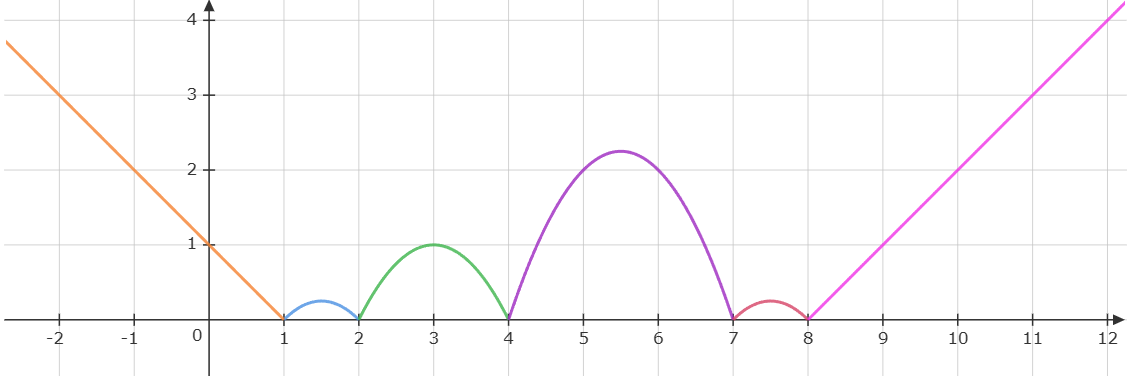
\includegraphics[width=0.8\textwidth]{psi.png}
  \caption{$\psi_i(w_i;\varepsilon)$ where $\varepsilon=0.2$ and $\mathcal{Q}_i=\{1,3,7,8,11\}$.}
  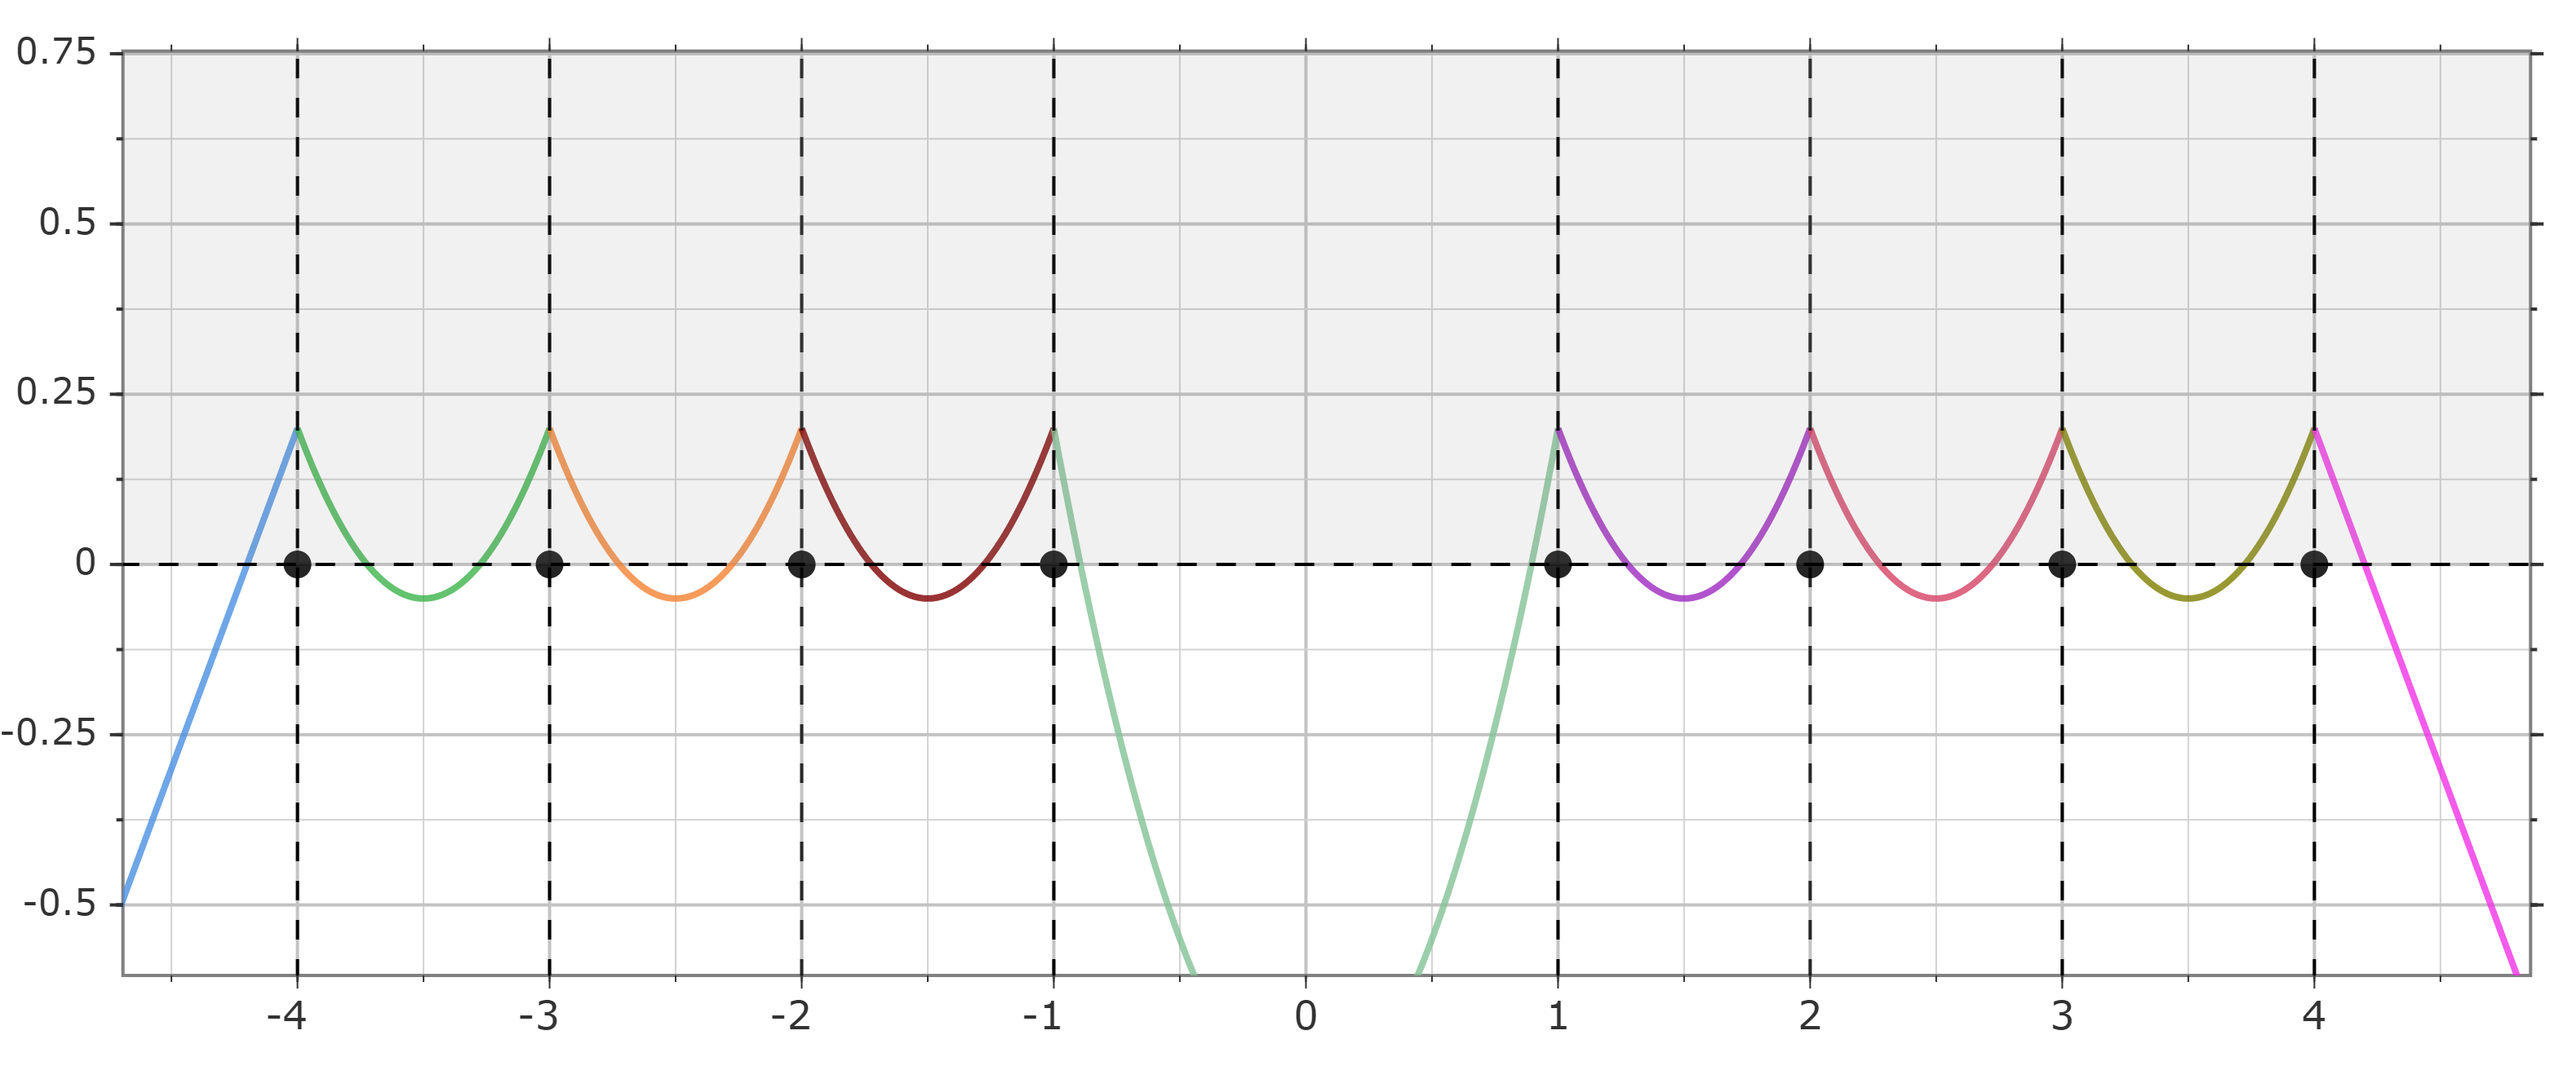
\includegraphics[width=0.8\textwidth]{psi2.png}
  \caption{The INT3 uniform quantization scheme, where $\varepsilon=0.2$ and $\mathcal{Q}_i=\{-4,-3,-2,-1,1,2,3,4\}$.}

\end{figure}

\newpage
\section{Experimental Results}

\textbf{Two Moons Classification}. We train a five-layer MLP (shown as below) with a 2-dimensional input, and ReLU as activation function on the non-convex two moon classification task for $T=60$ epochs. Our dataset consists of $n=2000$ training samples (in batches of $200$ per iteration, points are colored in blue and red) and $m=500$ test samples (color in black and white), which is generated by \texttt{scikit-learn} library's \texttt{make\_moons} data generator. We have also added a random Gaussian noise with the variance of $\xi=0.1$ to offset the point from its original position. We apply the logistic loss function in this experiment. The learning rate $lr$ and the hyperparameter for ASkewSGD $\alpha$ are set to $0.2$ and $0.2$, respectively.
\begin{figure}[H]
  \centering
  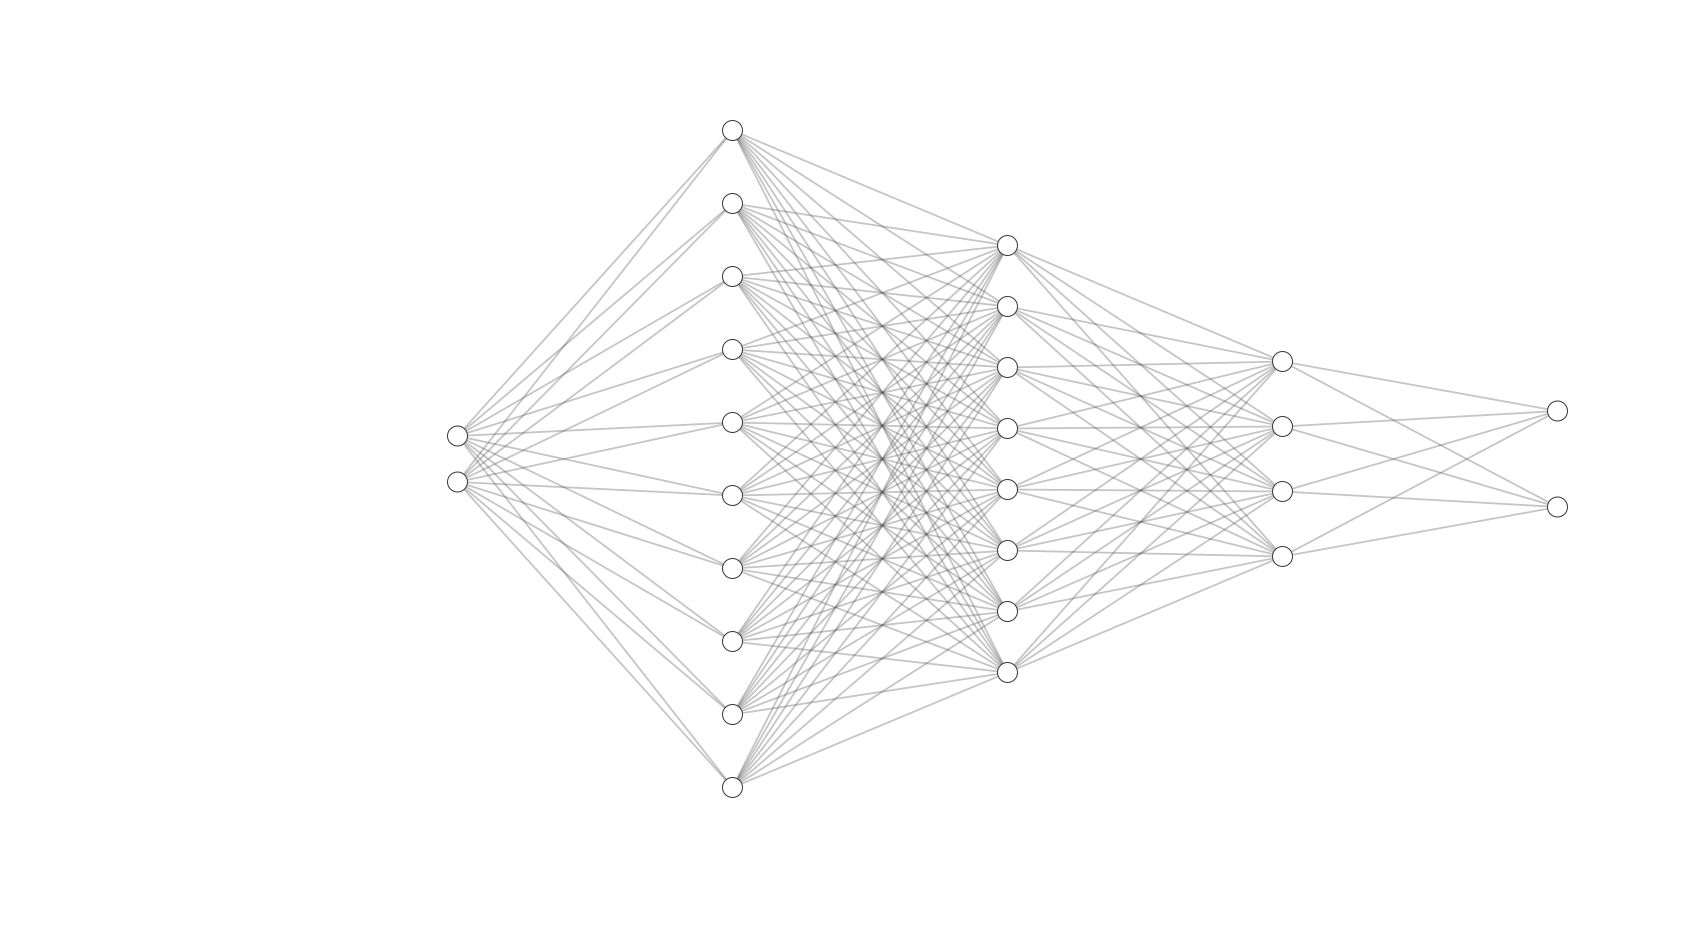
\includegraphics[width=0.6\linewidth]{nn.png}
\end{figure}

We compare SGD, BinaryConnect, and ASkewSGD to obtain the following results for the two moons classification problem. The first row shows the performance of different optimizers on the original net before quantization, and the second row depicts the quantized model with the quantization set $\mathcal{Q}=\{-1,+1\}$.

\begin{table}[H]
  \caption{Logistic loss after 60 epochs.} \label{Tb:tb1}
  \begin{center}
    \begin{tabular}{ccc}
      \hline
      Method                               & Loss             & Quantized Loss   \\ \hline
      Full Precision [W32/A32]             & 0.00002          & 0.59982          \\ \hline
      Deterministic BinaryConnect [W1/A32] & 0.57799          & 0.03260          \\
      \texttt{ASkewSGD} [W1/A32]           & \textbf{0.00367} & \textbf{0.00513} \\ \hline
    \end{tabular}
  \end{center}
\end{table}
\begin{figure}[H]
  \centering
  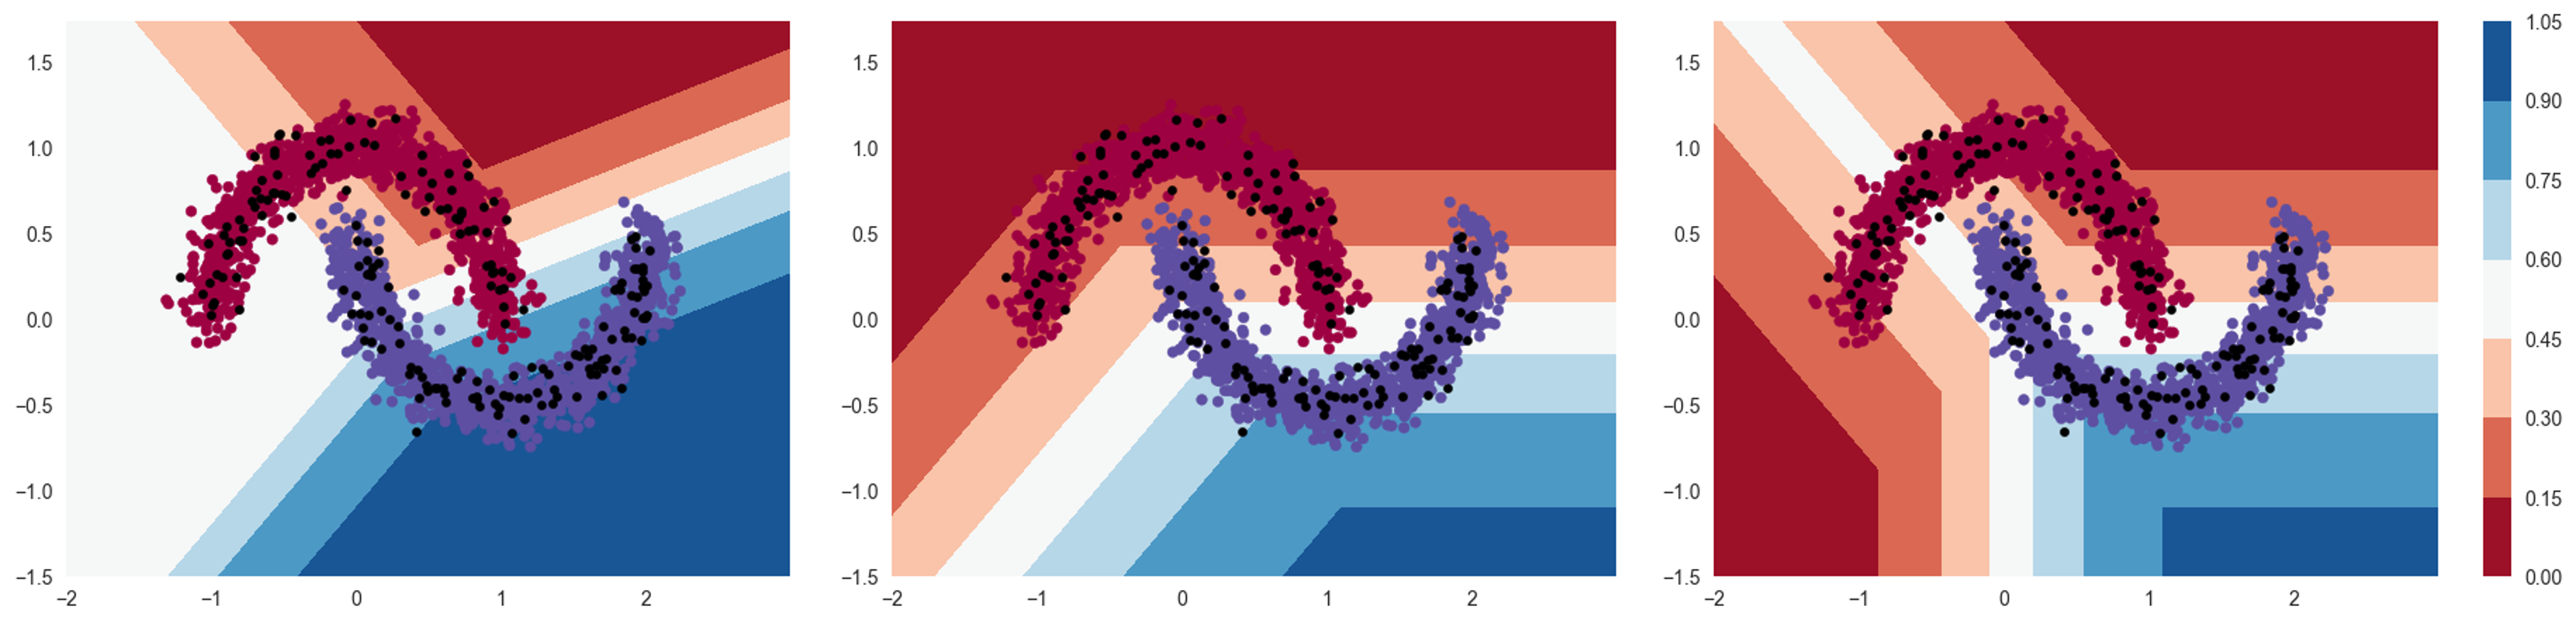
\includegraphics[width=0.7\linewidth]{../exp/twomoonstest.png}
\end{figure}
The original net has its contour completely perturbed by the weight quantization process. BinaryConnect is aware of the quantization scheme, thus generalizing well on the test set, but the original model is completely off from the groundtruth. ASkewSGD, on the other hand, has only a slight skew away from the sensible region, and the quantized model is still able to generalize well on the test set, which demonstrates the strength of this optimization method.

\newpage
\textbf{Computer Vision Task}. We train \texttt{ResNet-18} without bias and tunable parameters on the batch normalization layer on the CIFAR-10 dataset for $T=150$ epochs. The dataset consists of $n=50000$ training samples and $m=10000$ test samples. We apply the cross-entropy loss function in this experiment. We set the learning rate $lr$ and the hyperparameter for ASkewSGD $\alpha$ to $0.06$ and $0.2$, respectively. The quantization set $\mathcal{Q}$ is set to $\{-1,+1\}$.
\begin{figure}[H]
  \centering
  \includegraphics[width=0.9\linewidth]{../exp/CIFAR10_LO.png}
  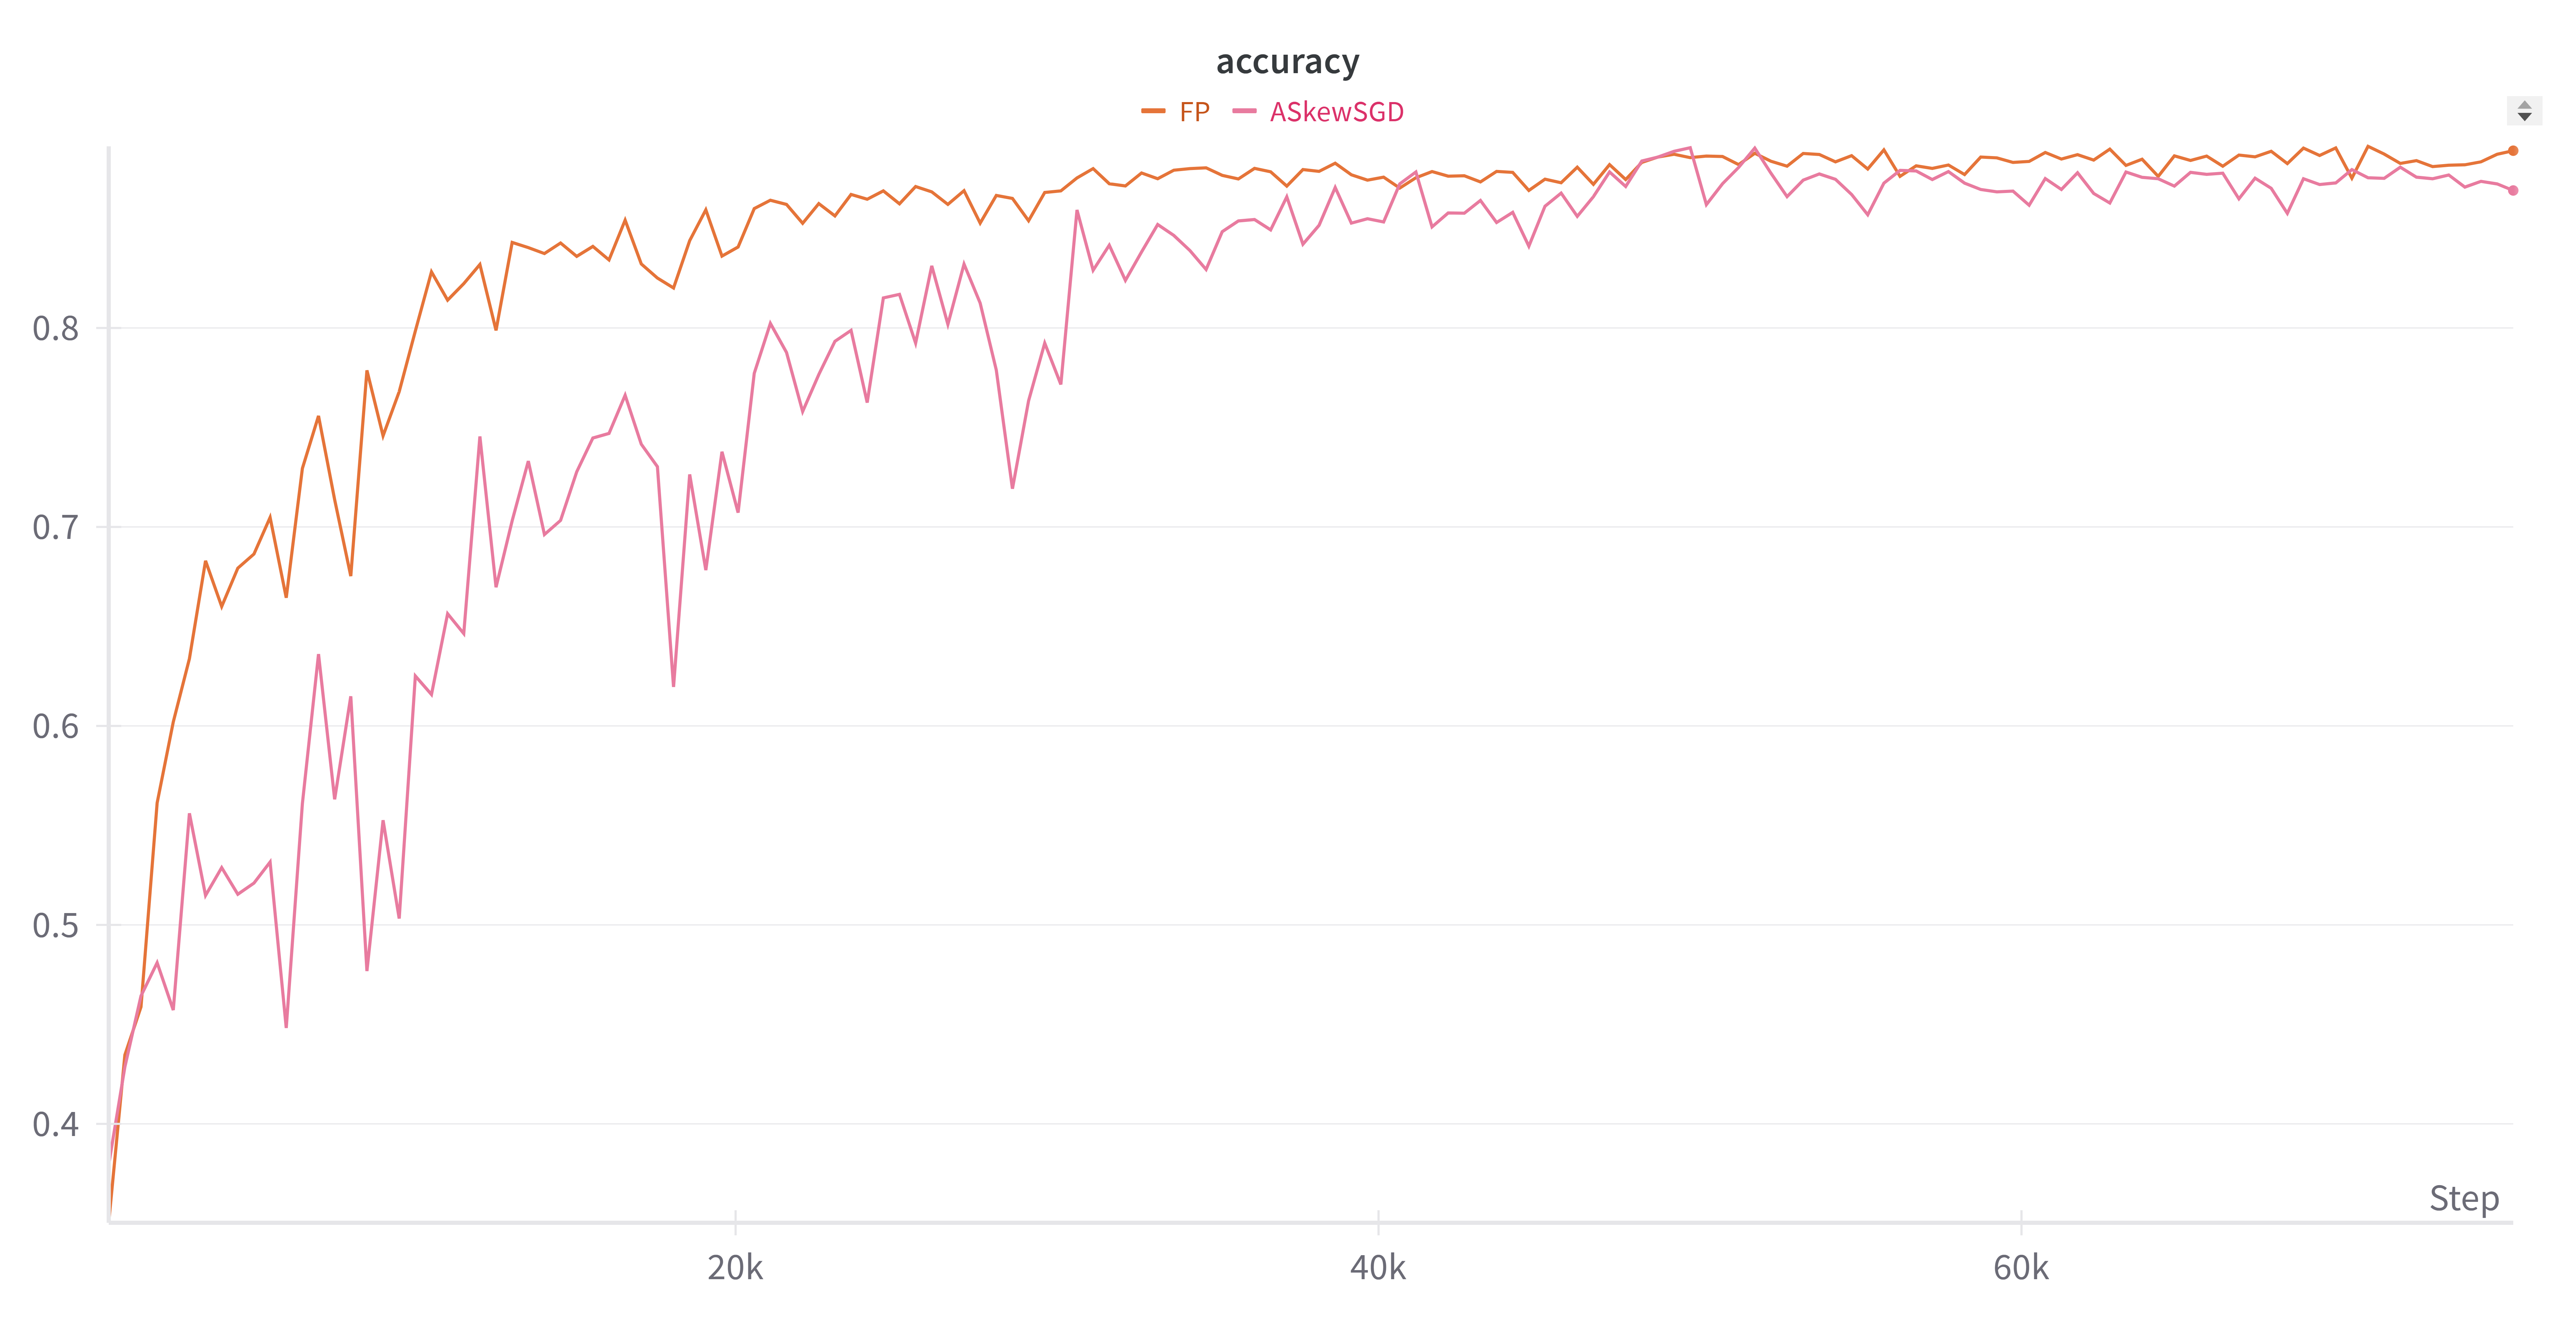
\includegraphics[width=0.45\linewidth]{../exp/CIFAR10_AC.png}
  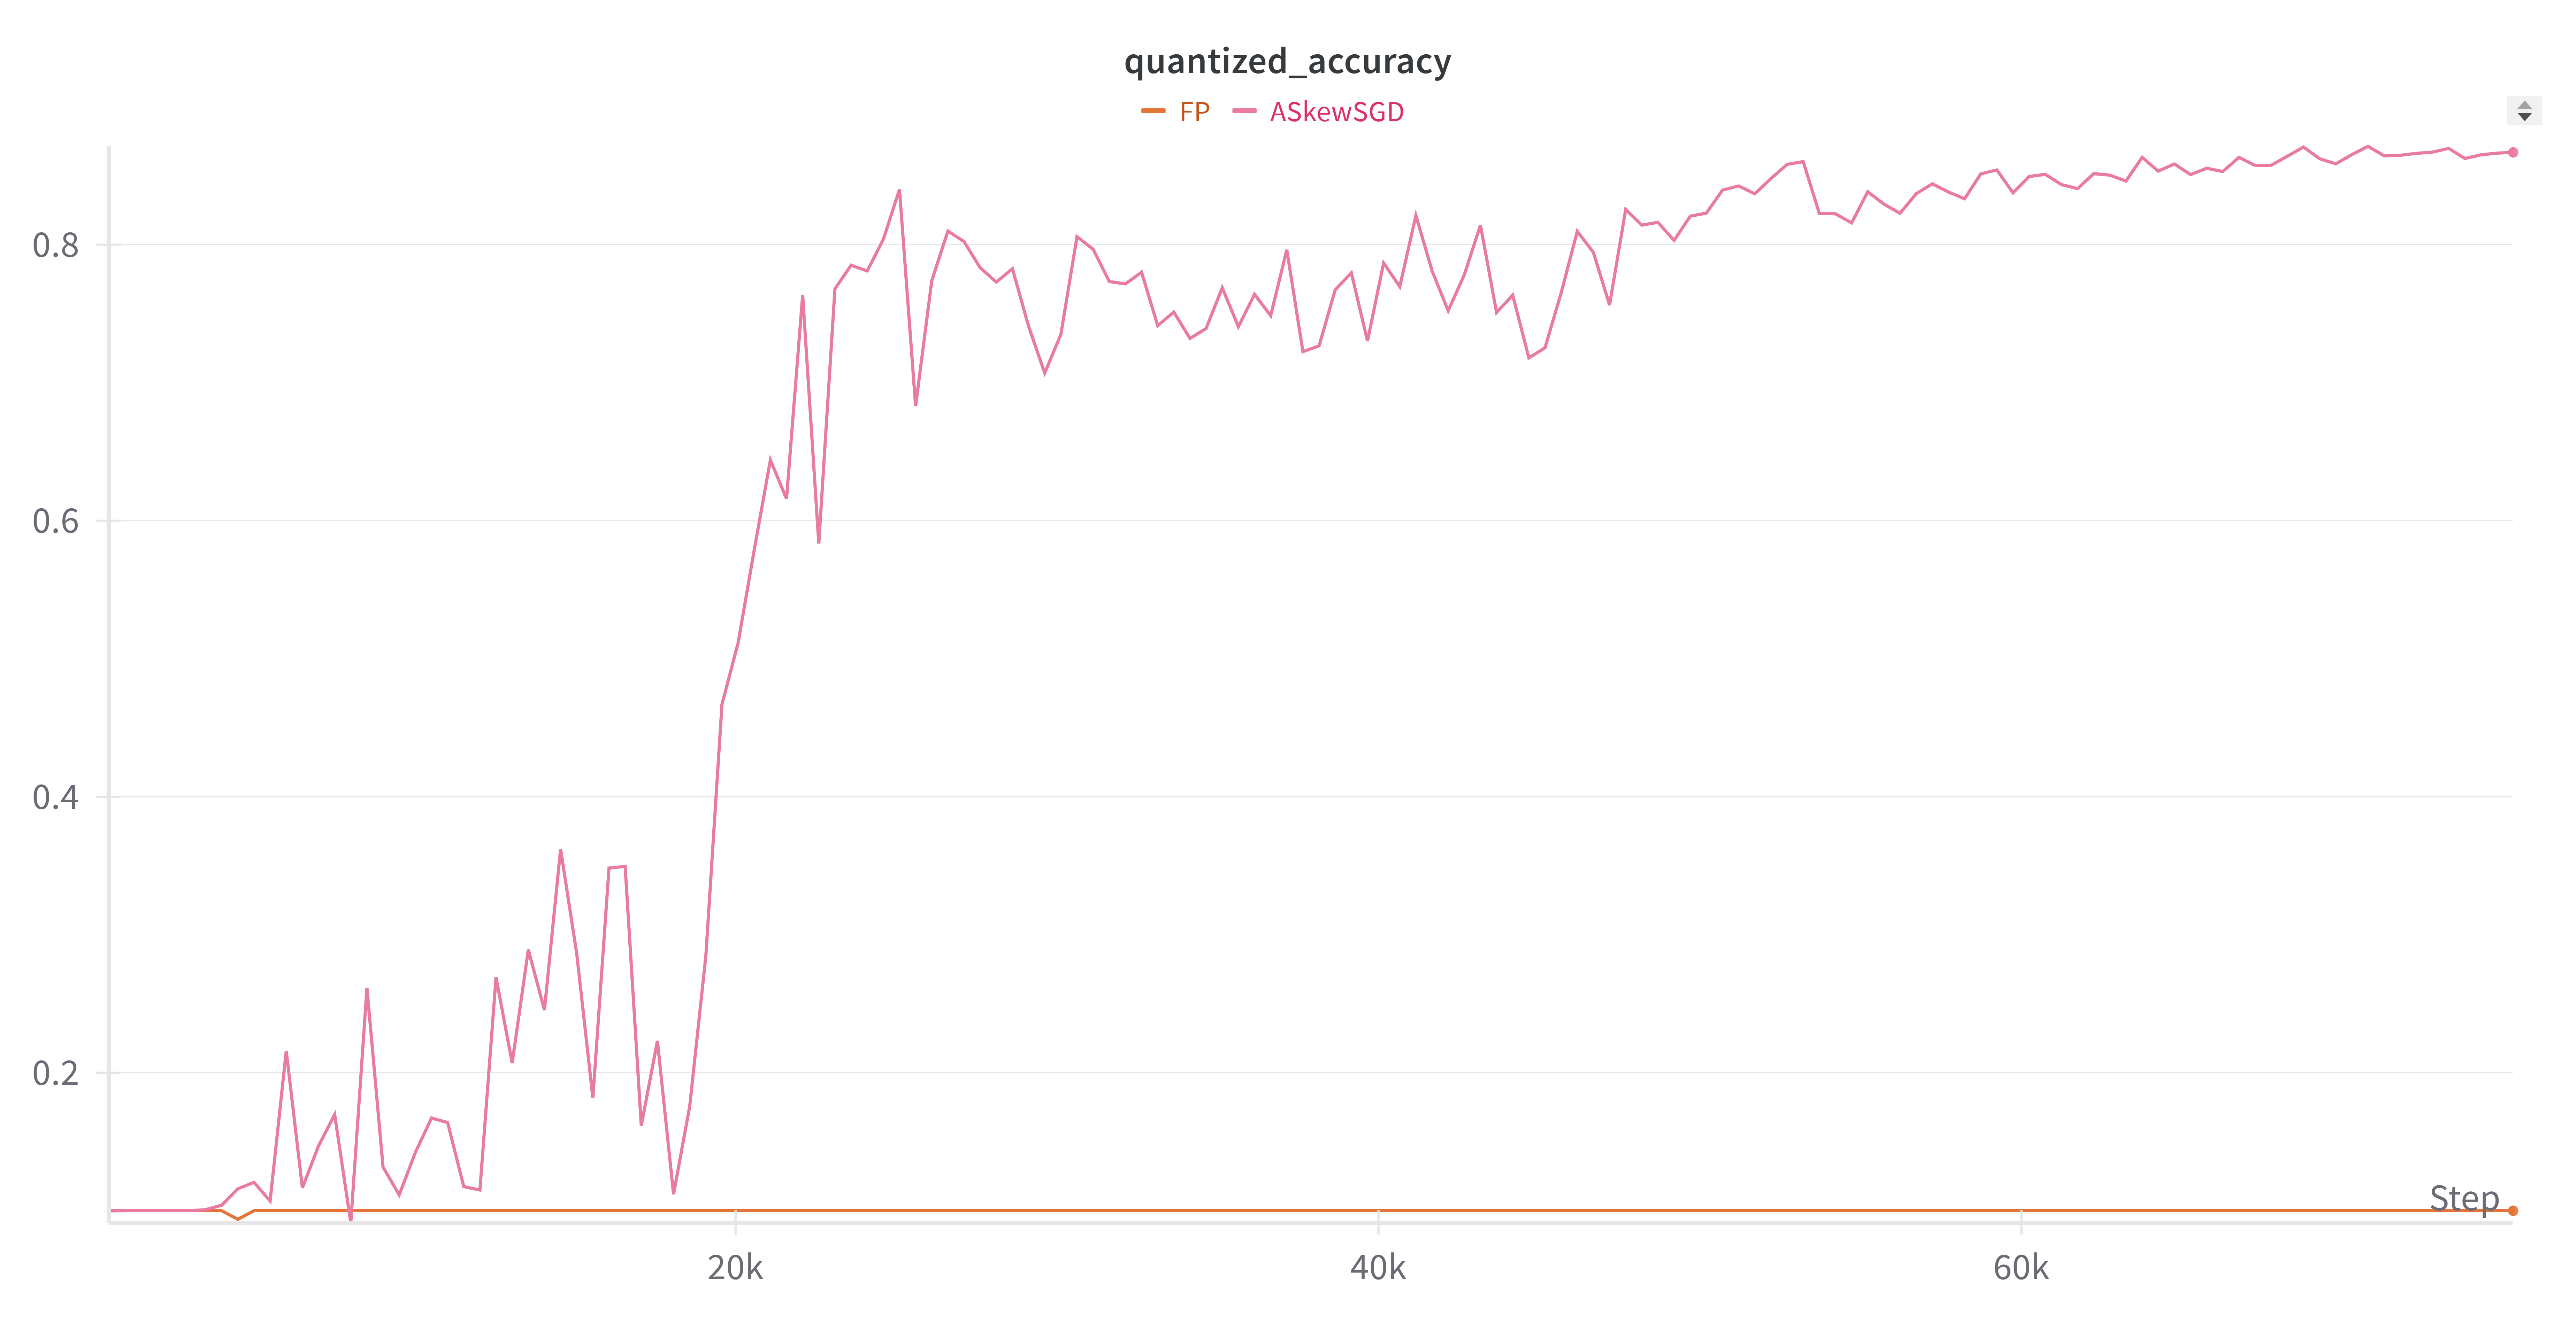
\includegraphics[width=0.45\linewidth]{../exp/CIFAR10_QA.png}
\end{figure}

\begin{table}[H]
  \caption{Performance of ResNet-18 on CIFAR10 after 60 epochs.} \label{Tb:tb1}
  \begin{center}
    \begin{tabular}{cccc}
      \hline
      Method                     & Accuracy & Loss    & Quantized Loss \\ \hline
      Full Precision [W32/A32]   & 88.91\%  & 0.04533 & 0.1            \\ \hline
      \texttt{ASkewSGD} [W1/A32] & 86.91\%  & 0.12337 & 0.8669         \\ \hline
    \end{tabular}
  \end{center}
\end{table}

It is worthwhile to note that the accuracy of the quantized model skyrocketed to $50\%$ only after running for 40 epochs, meaning that quantized models are sensitive to the accumulation of positional errors and the uncertain landscape of the loss function.

\newpage
\section{Comments}
\begin{enumerate}[label=\text{[}\arabic*\text{]}]
  \item The proof of Lemma 2 is not very clear. Remember to mark all assumptions in this Lemma, and fix a $K$ for the proof.
  \item Remember to write down the theorem statement of 3.1, clearly indicate the use of $\varepsilon$-$N$ where $\varepsilon$ is replaced by $\varepsilon_1$.
  \item Write the statement of 3.2, in the $(\varepsilon, \delta)$-stationary senses.
\end{enumerate}


\newpage
\section{References}
\begin{enumerate}[label=\text{[}\arabic*\text{]}]
  \item \label{1}L. Leconte, S. Schechtman and E. Moulines. (2023). ASkewSGD: An Annealed Interval-Constrained Optimisation Method to Train Quantized Neural Networks. In \textit{Artificial Intelligence and Statistics 2023}, \textbf{206}:3644-3663.
  \item \label{2}T. Dockhorn, Y. Yu, E. Sari, M. Zolnouri, V. P. Nia. (2021). Demystifying and Generalizing BinaryConnect. In \textit{35th Conference on Neural Information Processing Systems (NeurIPS 2021)}. \url{arxiv.org/pdf/2110.13220}.
  \item \label{3}M. Muehlebach, M. I. Jordan. (2022). On Constraints in First-Order Optimization: A View from Non-Smooth Dynamical Systems. In \textit{Journal of Machine Learning Research}, \textbf{23}(256):1-47. \url{http://jmlr.org/papers/v23/21-0798.html}.
  \item \label{4}S. Ghadimi, G. Lan. (2013). Stochastic First- and Zeroth-Order Methods for Nonconvex Stochastic Programming. In \textit{SIAM Journal on Optimization}, \textbf{23}(4):2341-2368.

\end{enumerate}

\end{document}